%\documentclass[fleqn]{book}
\documentclass[11pt]{amsbook}

\usepackage[turkish]{babel}

%\usepackage{../HBSuerDemir}	% ------------------------
\usepackage{../Ceyhun}	% ------------------------
\usepackage{../amsTurkish}


\begin{document}
% ++++++++++++++++++++++++++++++++++++++
\hPage{72}
% ++++++++++++++++++++++++++++++++++++++



\subsection{İKİ KÜMELİ ÇİZGELER}

 Ç(d,a) daki düğümlerin bir altkümesi  $\Delta_1 $ i düşünelim.
 Eğer bu kümedeki düğüm çiftlerinden 
 hiç biri birbirine bitişik değilse,
 bu kümeye \textit{ bağımsız küme} 
 diyeceğiz. Örneğin, Şekil 2.4.1'deki çizgede,
 
    $$
   \Delta_1 = \left(  d_1 \right)\quad
    \Delta_2 = \left(  d_1 ,d_3 \right) \quad
    \Delta_3 = \left(  d_1 ,d_3,d_4,d_6,d_7, d_9 \right)
     $$
kümeleri bağımsızdır.


     \begin{figure}[htb]
	    \centering
	    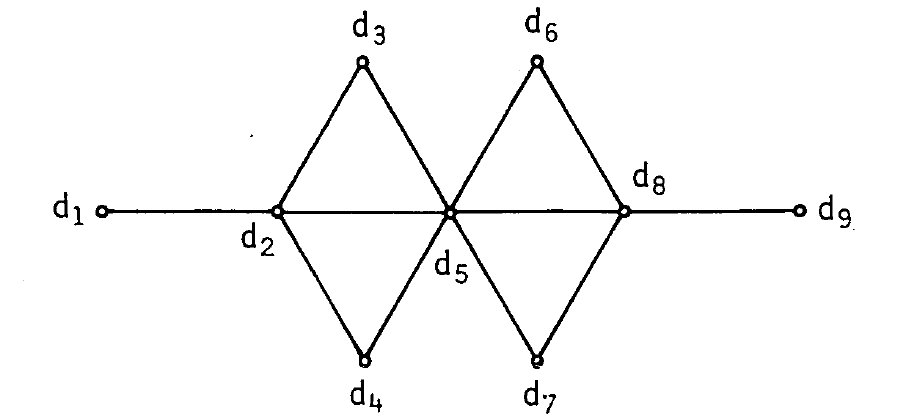
\includegraphics[width=0.9\textwidth]{images/ceyhun-072-Page-fig01}
	    \caption{Bağımsızlığın açıklanması.}
    	
    \end{figure}
    
    
    \begin{definition}{}
     Ç(d,a) da en çok düğümü içeren bağımsız kümedeki düğüm sayısına,çizgenin 
    \textit{\underline{ bağımsızlığı}} 
    $  \left(  \beta \right) $ denir.
	\end{definition}
    
Şekil 2.4.1 'deki çizgede en çok
düğümü içeren bağımsız küme  
$\Delta_3 $ 'dür.
Öyleyse,bu çizgenin bağımsızlığı altıdır.
$  \left(  \beta =6 \right) $

\end{document}